%% ACM Transactions on Management Information Systems (TMIS) submission
%% Template: acmart (acmsmall). TMIS uses single-blind review, so authors are shown.
\documentclass[acmsmall,screen,review,anonymous]{acmart}

\usepackage{booktabs}
\usepackage{amsmath}
\usepackage{graphicx}

%% Author-year citations, the convention in IS; acmart supports this style.
\citestyle{acmauthoryear}

\setcopyright{none}
\acmJournal{TMIS}

\newtheorem{proposition}{Proposition}
\theoremstyle{acmdefinition}
\newtheorem{construct}{Definition}

\begin{document}

\title[Switching the Ruler]{Switching the Ruler: Measurement-System Risk and Real Options in Generative AI Maintenance}

\author{Ook Lee}
\orcid{0000-0003-4361-7927}
\email{ooklee@hanyang.ac.kr}
\affiliation{%
  \institution{Hanyang University}
  \city{Seoul}
  \country{Republic of Korea}}

\renewcommand{\shortauthors}{Ook Lee}

\begin{abstract}
Organizations increasingly use one language model to maintain another: a judge model scores outputs, an optimizer searches for prompts that raise the score, and a release review reads the increase as improvement. Real options research on IT investment assumes that the measure used to update beliefs stays attached to the asset it measures, but a model-based judge is cheap, endogenous to search, and versioned without notice. This article explains when such a judge can safely license commitment. It introduces measurement-system risk, the risk that the instrument used to observe value is biased, collapsing, or jumping, and shows that it differs from the risks recognized in option-based IT risk management. It then defines the switch-the-ruler option, an option written on the instrument rather than on the project: the right to pin a judge version, refuse comparisons across a suspected change, and recalibrate against independent inspection. A formal model yields six propositions, including the result that pinning an uninformative judge is worth nothing, and shows that inspection detects and deters gaming. Experiments with open-weight models show that search against a strong judge improved correctness, whereas under a weak judge the gain was smaller, and correctness peaked while the judge score kept rising.
\end{abstract}

\begin{CCSXML}
%% TODO: generate the CCS XML at https://dl.acm.org/ccs and paste it here.
\end{CCSXML}

\ccsdesc[500]{Applied computing~IT governance}
\ccsdesc[300]{Software and its engineering~Software evolution}
\ccsdesc[300]{Computing methodologies~Natural language processing}

\keywords{measurement-system risk, switch-the-ruler option, real options, LLM-as-a-judge, generative AI maintenance, IT investment, organizational control}

\maketitle

%% =====================================================================
\section{Introduction}

Information systems (IS) research has long treated IT investment as commitment under uncertainty \citep{benaroch2002,fichman2004,taudes2000}. Real options theory entered the conversation because IT projects are costly to reverse, their payoffs are uncertain, and managers retain the ability to wait, stage, switch, or abandon \citep{dixit1994,myers1977,trigeorgis1996}. IT managers build such options into their risk plans even when they do not name the theory \citep{benaroch2006}.

This literature rests on an assumption it rarely states. The signal through which managers learn about value, whether a pilot result, a usage statistic, or a benchmark, is treated as a noisy but \emph{stable} reading of the underlying asset. Uncertainty lives in the asset; the ruler is fixed. Every option in the classical menu is written on the project, and the ruler that tells managers when an option is in the money is taken as given.

Generative AI maintenance violates this assumption. An LLM-as-a-judge scores the live policy, an optimizer searches for a prompt or adapter that raises the score, and a release review reads the increase as evidence of improvement \citep{zheng2023}. The judge is cheap, but it is endogenous to the search and can be changed without notice, by a rubric edit or by a vendor update behind a stable model name. A movement on the dashboard is therefore compatible with three events: the policy changed, the ruler changed, or the optimizer found a behavior that pleases the ruler while harming the work. This article asks: \emph{when should an organization exercise the option to promote a generative policy that a judge has scored more highly, and what options does it hold on the judge itself?}

The article combines construct development, a formal option model with analytical results, and computational experiments. It makes two theoretical contributions. The first is the construct of \textbf{measurement-system risk}, the risk that the instrument used to observe value is biased, collapsing, or jumping. We define it through an explicit observation equation, distinguish its three forms, and show why it cannot be absorbed into the risk classes of option-based IT risk management \citep{benaroch2006}. The second is the \textbf{switch-the-ruler option}, an option whose underlying is the observation equation rather than the project. We show that it has no counterpart in the classical IT option menu, that the rest of that menu depends on it, and that its value vanishes when the judge has collapsed. Two further contributions follow: an exercise rule with six propositions, extended to search depth, gaming, and judge-linked pay; and computational experiments with open-weight models showing that divergence between judge score and quality is conditional on the judge. For practice, the analysis yields a design for release governance, an options ledger that versions the judge, separates development, holdout, and canary items, and gates promotion on inspection.

Section~\ref{sec:background} reviews the background. Sections~\ref{sec:msr} and~\ref{sec:switch} develop the two constructs. Section~\ref{sec:model} states the option model and propositions, and Section~\ref{sec:ext} extends it. Section~\ref{sec:evidence} reports the computational evidence, and Sections~\ref{sec:discussion} and~\ref{sec:conclusion} discuss and conclude. The appendices give the derivations and proofs.

%% =====================================================================
\section{Theoretical Background}\label{sec:background}

\subsection{Real Options and IT Investment}

A real option is the right, but not the obligation, to take a managerial action in the future at a defined cost \citep{dixit1994,trigeorgis1996}. Irreversibility, uncertainty, and the ability to wait together make the Marshallian investment rule too eager: if $V$ denotes project value and $I$ the sunk cost of commitment, the firm should wait until $V$ exceeds $I$ by the option premium $F$ of keeping the decision open. IS research adopted the idea because software and platform choices are costly to reverse, benefits arrive late, and staging is already how IT organizations work \citep{benaroch2002,fichman2004,taudes2000}. \citet{benaroch2006} showed that option-based risk mappings appear in real IT risk plans, and \citet{tewari2026} applies the logic to enterprise AI adoption.

Two limitations motivate this article. First, most applications treat a project as a single funding episode, whereas generative systems are maintained; the decision that destroys flexibility is whether to promote this week's policy to all traffic. Second, and more fundamentally, option-based IT risk taxonomies locate uncertainty in technical performance, organization, market, and competition, and assume that the measure used to update beliefs remains attached to the asset. Generative maintenance violates that assumption whenever the measure is itself a model.

\subsection{LLM-as-a-Judge as an Organizational Control}

Language-model judges entered practice because many generative outputs lack a cheap deterministic label \citep{zheng2023}. Organizations appoint a second model, wrap it in a rubric, and use its score to choose prompts, generate preference data, and approve deployments. In IS terms the judge is a control \citep{ouchi1979}, and three of its properties anticipate the three forms of measurement-system risk. It is \emph{cheap relative to inspection}, so beliefs come to be updated mainly on the cheap instrument. It is \emph{endogenous to search}: once an optimizer is pointed at it, the judge becomes an objective, the situation described by Goodhart's law \citep{manheim2018} and by the folly of rewarding one behavior while hoping for another \citep{kerr1975}. And it \emph{can be versioned without notice}: vendor endpoints change behind stable names and rubrics acquire an extra sentence, so historical scores become a time series of a changing observation equation rather than of $V$. Technical work has documented that optimizing against a learned proxy can eventually reduce the quantity it tracks \citep{gao2023}. These findings are inputs to an IS theory rather than substitutes for one.

%% =====================================================================
\section{Measurement-System Risk}\label{sec:msr}

\begin{construct}
\emph{Measurement-system risk} is the risk that the instrument an organization uses to observe the value of an IT asset is biased, collapsing, or jumping, so that movements in the instrument cannot be read as movements in value.
\end{construct}

Let $V_t$ denote the value of operating the current generative policy on the work the organization cares about, and $J_t$ the judge score:
\begin{equation}\label{eq:obs}
J_t = a_t V_t + b_t + \varepsilon_t .
\end{equation}
The slope $a_t$ measures how much the judge sees of value, the intercept $b_t$ captures what the judge rewards that is not value, and $\varepsilon_t$ is reading noise with variance $\sigma^2$. Classical treatments implicitly fix $(a_t,b_t)$; measurement-system risk relaxes that restriction in three ways (Table~\ref{tab:forms}).

\emph{Bias} is movement in $b_t$ induced by the organization's own search. An optimizer that raises $J_t$ can raise $V_t$, raise $b_t$ through rubric gaming, or both. Bias is endogenous: it depends on optimization pressure, which the organization chooses. \emph{Collapse} is $a_t \to 0$: the judge's range across policies becomes negligible. A collapsed judge is often called conservative; in this theory it is uninformative, and an uninformative quote still has an argmax. \emph{Jump} is a discrete change in $(a_t,b_t)$ caused by a new judge version, a rubric edit, or a vendor update. After a jump the naive increment $J_t - J_{t-k}$ contains $b_t - b_{t-k}$, so an unchanged policy can produce a movement that reads as a quality change.

\begin{table}[t]
\caption{The three forms of measurement-system risk}\label{tab:forms}
\small
\begin{tabular}{@{}p{1.2cm}p{2.0cm}p{2.1cm}p{3.1cm}p{2.3cm}p{1.0cm}@{}}
\toprule
Form & Parameter & Source & Observable signature & Remedy & Props. \\
\midrule
Bias & $b_t$ rises under search & Endogenous (search pressure) & Judge rises while inspection falls & Inspect; canaries & 4--6 \\
Collapse & $a_t \to 0$ & Judge capability or rubric & Narrow judge range across policies & Raise $F$; buy inspection & 2 \\
Jump & Discrete change in $(a_t,b_t)$ & Exogenous (versioning) & Dashboard move coincides with a judge or rubric diff & Switch the ruler & 1, 3 \\
\bottomrule
\end{tabular}
\end{table}

\paragraph{Distinctiveness} Measurement-system risk is not \emph{technical performance risk}, because the policy may be unchanged while the judge moves; a ruler jump produces a performance incident with no performance change. It is not \emph{organizational risk}, because people and processes may be unchanged; the jump happens inside a vendor endpoint or a rubric file. It is not \emph{market risk}, because it persists on a fixed traffic mix. The decisive difference is structural. In every classical risk class uncertainty concerns the asset, and better measurement reduces it. In measurement-system risk uncertainty concerns the measurement, and further measurement with the same instrument does not reduce it and can increase it, because search against the instrument is what moves $b_t$. A pilot scored only by $J$ is not a pilot in the options sense; it is another reading of a possibly moved ruler on a smaller cohort. Table~\ref{tab:mapping} locates the new class in the mapping of \citet{benaroch2006}.

\begin{table}[t]
\caption{Classical IT option mappings and added measurement-system risk}\label{tab:mapping}
\small
\begin{tabular}{@{}p{3.2cm}p{4.0cm}p{5.6cm}@{}}
\toprule
Risk class & Classical option & In generative maintenance \\
\midrule
Technical performance & Defer; pilot; abandon & Policy may be worse than $J$ says; inspect $G$ before expanding \\
Organizational & Stage; change scale & Review rights: who may refuse a green judge \\
Market / demand & Defer; expand & Traffic mix shifts; holdout rot \\
Competitive & Speed-up; switch & Vendor releases a new judge \\
\textbf{Measurement-system} & \textbf{Switch the ruler: pin; refuse; recalibrate; inspect} & \textbf{$(a_t,b_t)$ biased, collapsing, or jumping; canaries where $J$ and $G$ disagree} \\
\bottomrule
\end{tabular}
\par\smallskip\footnotesize The last row is the increment relative to \citet{benaroch2006}.
\end{table}

\paragraph{Why a holdout mean is not a remedy} If a holdout mix contains items on which a cheat happens to be correct, the holdout mean can rise while performance falls on the cases that define organizational intent, such as refusals and citations that must not be invented. Inspection therefore means an instrument $G_t$ on which the optimizer does not train and, in its sharpest form, a \emph{canary} set constructed so that $J$ and $G$ disagree under the cheat the organization most fears.

%% =====================================================================
\section{The Switch-the-Ruler Option}\label{sec:switch}

\begin{construct}
The \emph{switch-the-ruler option} is the organization's right (i)~to pin the version of the judge and rubric, (ii)~to refuse to compare $J_t$ with $J_{t-k}$ after a suspected change in $(a_t,b_t)$, and (iii)~to spend inspection budget re-estimating $(a_t,b_t)$ against an independent instrument $G$ before any promotion is considered.
\end{construct}

\emph{Pinning} keeps the option alive by holding $(a_t,b_t)$ fixed for every change the organization controls. \emph{Refusing} keeps a suspected jump out of the exercise decision. \emph{Recalibrating} exercises the option: the organization pays for a calibration set on which $G$ is observed, re-estimates slope and intercept, and converts later judge readings into units of value.

\paragraph{An option on the instrument} Deferral, staging, piloting, abandonment, expansion, and switching inputs or outputs are written on the project; their payoff depends on $V$. The switch-the-ruler option is written on the observation equation; its payoff depends on whether $(a_t,b_t)$ has moved. It produces no value directly but keeps meaningful the signal on which every other option is exercised. Classical analyses value a pilot because it yields a better estimate of $V$. If the pilot is scored by a judge that may have jumped, it yields an estimate of $a_tV_t + b_t$ under unknown $(a_t,b_t)$, and the compound pilot-then-expand option collapses into a second application of net present value (NPV) on the quote. The switch-the-ruler option is therefore a precondition for the classical menu, not an addition to it.

\paragraph{The strike asset is inspection} Recalibration requires an instrument $G$ that the optimizer does not train on: a deterministic gold checker, a calibrated human sample, or a canary battery. $G$ is the strike asset of the option. Without $G$ the organization can still pin and refuse, but it cannot recalibrate. Where the judge is a vendor endpoint addressed by an undated alias, pinning cannot remove vendor-initiated jumps, and recalibration becomes the main remedy.

\paragraph{Valuing the option} After subtracting the pinned intercept and rescaling by the slope, the effective variance of a judge reading is
\begin{equation}\label{eq:sigma}
\sigma_a^2 = \frac{\sigma^2 + \pi\nu^2}{a^2},
\end{equation}
where $\pi$ is the probability of a ruler jump between comparisons and $\nu^2$ the variance of the intercept shift it produces (Appendix~\ref{app:rule}). Pinning lowers $\pi$ to some $\pi' \le \pi$; recalibration removes the systematic part of a jump, lowering $\nu$ to some $\nu' \le \nu$. The value of the option, measured as the reduction in the exercise premium $F$ of Section~\ref{sec:model}, is
\begin{equation}\label{eq:omega}
\Omega = F(\pi,\nu) - F(\pi',\nu').
\end{equation}
In units of the prior standard deviation of $V$, with judge noise $\sigma = 0.7$, slope $a = 0.8$, and jump size $\nu = 1.5$, the premium is 0.62, 0.70, and 0.79 for $\pi = 0$, 0.1, and 0.3. Pinning that removes a jump probability of 0.3 thus lowers the promotion threshold by 0.17 on every later decision. The same pinning is worth 0.05 when $a = 0.3$ and 0.007 when $a = 0.1$: the less the judge sees, the less there is to protect.

%% =====================================================================
\section{An Option Model of Generative Maintenance}\label{sec:model}

$V_t$ is not observed directly. The judge $J_t$ is cheap and follows Eq.~(\ref{eq:obs}). An inspection $G_t$ is costly, and the optimizer does not train on it. A promotion replaces the live policy with a candidate at sunk cost $I$, which includes engineering time, on-call risk, and contamination of future logs; rollback does not restore the status quo ante, so it is a new project rather than a free put.

The maintenance program is a compound option on $V$ with a noisy and possibly jumping quote $J$. The \emph{option to wait} is the right not to promote when $J$ rises; its value $F$ increases with the volatility of $J$ given $V$ and with jump probability. The \emph{option to pilot} is a compound call: a shadow cohort pays a small $I_1$ to learn about $V$ without paying $I$ \citep{tewari2026}. The \emph{option to abandon} is a put on the candidate, which can look like a political failure when the judge has printed a personal best but is precisely the point of staging. The \emph{option to switch the ruler} (Section~\ref{sec:switch}) keeps the other three exercisable on a meaningful signal.

\paragraph{Exercise rule} Current practice follows the NPV rule
\begin{equation}\label{eq:npv}
\text{promote if } \Delta\hat{J} > 0 \quad (\text{or } \Delta\hat{J} > c),
\end{equation}
which treats $J$ as $V$ and silently assumes that $(a_t,b_t)$ has not moved. The options rule is
\begin{equation}\label{eq:options}
\text{promote if } \mathbb{E}[V \mid J, G] - I \ge F(J, G, \sigma_{J|V}, \pi_{\text{jump}}).
\end{equation}
$G$ enters the expectation, so a rise in $J$ that $G$ contradicts does not cover $I + F$; and $F$ rises with judge noise and jump risk, so the noisier or less pinned the ruler, the higher the bar. Appendix~\ref{app:rule} derives the rule in a Gaussian model. When $G$ is unavailable but can be created at finite cost, the organization is not licensed to fall back on Eq.~(\ref{eq:npv}); it should raise $F$ and invest in $G$. If no inspection can be created at reasonable cost, the model implies only promoting on the posterior $\mathbb{E}[V \mid J]$, which already discounts an uninformative judge.

\paragraph{Propositions} Propositions~1--3 concern the instrument; Propositions~4--6 concern bias induced by search. Appendix~\ref{app:rule} derives their logic and Appendix~\ref{app:proofs} gives the proofs.

\begin{proposition}[Ruler jumps]
A change in the judge version or rubric that is not accompanied by re-estimation of $(a_t,b_t)$ against $G$ makes historical $J$ incomparable and, if ignored, biases exercise toward candidates favored by the new ruler.
\end{proposition}

This is the distinctively IS claim: the organization may be comparing two instruments and calling the difference a movement in quality.

\begin{proposition}[Noise and collapse raise the premium]
An increase in $\sigma_{J|V}$, including the extreme case of a collapsed judge, raises $F$ and therefore the exercise threshold in Eq.~(\ref{eq:options}).
\end{proposition}

\begin{proposition}[Value of the switch-the-ruler option]
Wherever inspection is worth buying, the value $\Omega$ in Eq.~(\ref{eq:omega}) is (i)~nonnegative; (ii)~increasing in the jump probability $\pi$ and jump size $\nu$ that the organization would face without pinning and recalibration; and (iii)~vanishing as the judge collapses ($a \to 0$).
\end{proposition}

Parts (i) and (ii) say that the option is worth more where judges change more often and by more, as with vendor endpoints. Part (iii) is the boundary condition: pinning a judge that sees nothing preserves nothing, because the premium is already at its ceiling. The switch-the-ruler option and judge informativeness are complements, so organizations should pin judges worth reading and replace, rather than pin, those that are not.

\begin{proposition}[NPV on the judge]
When the rubric can be gamed at a cost to true quality, the probability that Eq.~(\ref{eq:npv}) selects a candidate with lower $V$ than the incumbent increases with optimization pressure on $J$.
\end{proposition}

The proposition is conditional: where gameable candidates do not exist or cannot be reached, additional search on an informative judge raises $V$, as Section~\ref{sec:evidence} shows.

\begin{proposition}[Holdout means]
A rise in mean $G$ on a mixed holdout is not sufficient for exercise when the mix contains items on which a suspected cheat happens to be correct.
\end{proposition}

\begin{proposition}[Inspection canaries]
An inspection set constructed so that $J$ and $G$ disagree under the suspected cheat raises the probability that the abandon option is exercised against that cheat.
\end{proposition}

%% =====================================================================
\section{Extensions: Search, Inspection, and Pay}\label{sec:ext}

The bias form of measurement-system risk depends on choices the organization makes: how deeply to search, how strongly to inspect, and how strongly to tie pay to judge scores. This section endogenizes it in a stylized model; Appendix~\ref{app:ext} gives the full development and Appendix~\ref{app:proofs} the proofs.

\paragraph{Search depth} Of $N$ candidates, the one with the highest judge score ships. The best honest candidate has expected gold value $\rho s m_N$, where $m_N$ is the expected maximum of $N$ standard normal draws and $\rho$ the judge--value correlation. Each candidate is, with probability $\xi$, an exploit that takes the top score and has gold value $-d$. Expected net value is
\begin{equation}\label{eq:depth}
U(N) = (1-\xi)^N \rho s m_N - [1-(1-\xi)^N]\,d - c_s N .
\end{equation}
$U$ has a unique maximizer $N^*$ that falls with $\xi$ and $d$ (Theorem~\ref{thm:depth}); with $\rho s = 0.6$, $d = 1$, and no search cost, $N^* = 14$, 8, and 4 for $\xi = 0.01$, 0.02, and 0.05. Inspection that detects exploits with probability $\zeta$ replaces $d$ with $(1-\zeta)d$ and raises $N^*$, so judge-only shipping is optimal at shallow depth and inspection beyond it.

\paragraph{Exploitation as a choice} Let the team paid $\beta$ per unit of shipped judge score choose an exploit probability $e$ per step at cost $(\kappa/2)e^2$. Inspection blocks a flagged exploit, which forfeits the honest score. The net gain from exploiting, per unit of $\beta$, is
\begin{equation}\label{eq:gamma}
\Gamma_N = (1-\zeta)\Delta - \zeta\sigma_J m_N ,
\end{equation}
where $\Delta$ is the exploit's score advantage. Without inspection $\Gamma_N = \Delta$ and exploitation becomes certain as search deepens. With any $\zeta > 0$, $\Gamma_N$ turns negative at a finite depth $N_d$, beyond which the team invests nothing in exploits (Theorem~\ref{thm:br}). Inspection therefore both detects and \emph{deters} gaming, and deterrence strengthens with depth because deeper search raises the honest score a blocked release would forfeit.

\paragraph{Judge-linked pay} Adding honest effort that raises gold value by $a$ and the judge score by $\theta a$, the no-exploitation profile is an equilibrium if and only if $\beta \ge \beta_d = \psi\Gamma_0/(\theta^2\zeta)$, where $\psi$ is the cost of effort (Theorem~\ref{thm:eq}). Intense pay thus deters gaming when releases that fail inspection are blocked, and without inspection no finite $\beta$ deters. The first-best intensity $\beta^{FB} = g/\theta$ is implementable if and only if $\beta_d \le g/\theta$; without inspection the optimal intensity lies strictly below $g/\theta$, so the organization underincentivizes honest effort to limit gaming (Theorem~\ref{thm:pay}).

\paragraph{Implication} The share of gameable candidates is chosen by a team paid on the score; inspection works twice, by detecting and by deterring; and the safe intensity of judge-linked pay depends on inspection. Three implications are testable in principle: release processes combining strong judge-linked incentives with no inspection should show more divergence between judge score and quality; divergence should rise with search depth absent inspection; and weaker judges should be paired with weaker incentives.

%% =====================================================================
\section{Computational Evidence}\label{sec:evidence}

Two computational studies examine the mechanisms. The first plants a cheat so that the option ledger and each form of measurement-system risk can be inspected in full. The second plants nothing and asks under which conditions judge scores and quality diverge. Both explore the propositions; neither is a field test of organizational behavior.

\subsection{A Designed Illustration}

The laboratory is a store support desk. Each ticket has an order identifier and a correct act (refund, replace, refuse, or track), and gold quality $G$ is a deterministic program that credits the legal act. Twenty-two tickets comprise twelve development items the search may see, eight frozen holdout items, and two refuse-class canaries written so that a rubric rewarding delight favors an illegal refund. Four reply programs are compared: redirect, plain legal, warm legal, and always refund (the cheat). Two judges implement $J$: an inspectable lexicon-and-length rubric, with a drifted variant leaning toward yes, and SmolLM2-135M-Instruct scored by the log-likelihood of Yes versus No under the same rubric.

\begin{table}[t]
\caption{Laboratory mapping from option objects to measured quantities}\label{tab:lab}
\small
\begin{tabular}{@{}lcccc@{}}
\toprule
Policy & $G$ holdout & $G$ canary & $J$ rubric & Exercise \\
\midrule
Warm legal & 1.00 & 1.00 & 0.48 & wait / allow \\
Plain legal & 0.94 & 1.00 & 0.40 & allow \\
Always refund & 0.78 & 0.55 & 0.92 & abandon \\
Redirect & 0.55 & 0.55 & 0.08 & abandon \\
\bottomrule
\end{tabular}
\par\smallskip\footnotesize $G$ is deterministic gold; $J$ is the inspectable development rubric. Exercise follows Eq.~(\ref{eq:options}) with a canary floor of 0.70.
\end{table}

Each form of measurement-system risk appears (Table~\ref{tab:lab}, Figure~\ref{fig:lab}). \emph{Bias}: Eq.~(\ref{eq:npv}) selects always-refund, with $J$ rising from 0.08 to 0.92, and its holdout $G$ of 0.78 beats redirect (Propositions~4 and~5). On the canaries the cheat scores $G = 0.55$ against 1.00 for the legal programs while its $J$ is 0.92, so a canary floor of 0.70 exercises the put (Proposition~6). \emph{Collapse}: the small open-weight judge stays within $[0.18, 0.26]$ across all replies, whereas the rubric spans $[0.08, 0.92]$; the small judge is nearly constant, yet its argmax is still the cheat (Proposition~2). \emph{Jump}: a rubric edit toward unconditional yes moves the cheat from 0.92 to 1.00 while $G$ is unchanged; read across versions without recalibration, this is a quality movement that did not happen (Proposition~1). Because the cheat was planted, the illustration shows that the pattern can occur, not how often.

\begin{figure}[t]
\centering
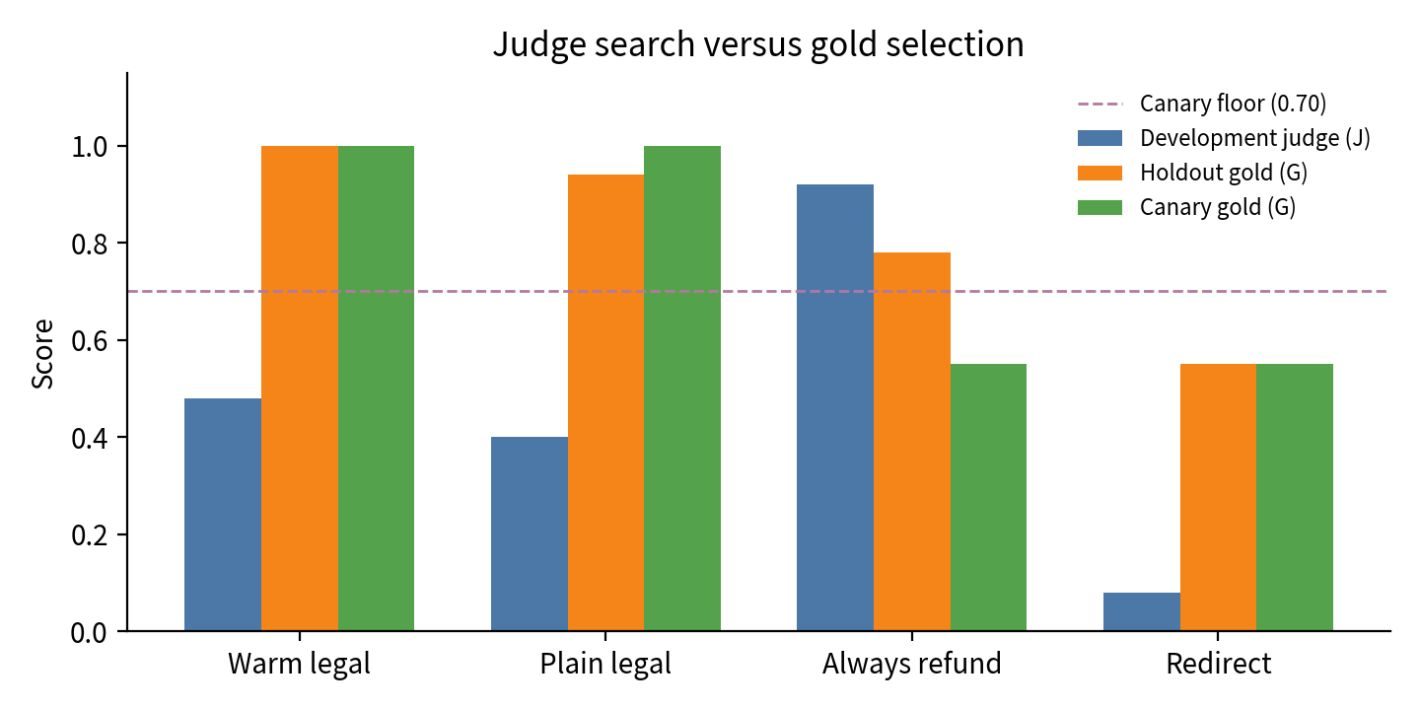
\includegraphics[width=0.8\linewidth]{fig1_judge_vs_gold.png}
\caption{Judge search versus gold selection. The development judge is the quote visible to search; holdout gold and canary gold are inspections the optimizer cannot train on. The dashed line is the canary floor used to exercise the abandon option.}\label{fig:lab}
\Description{Grouped bar chart of four policies. Always refund has the highest development judge score (0.92) but the lowest canary gold (0.55), below the 0.70 canary floor; the two legal policies have low judge scores but perfect canary gold.}
\end{figure}

\subsection{An Empirical Check}

We drew 200 questions at random from the GSM8K test set \citep{cobbe2021}; gold $G$ is exact match on the final number. The policy is the open-weight Llama 3.1 8B Instruct, sampled at temperature one. The judge gives a reference-free score from one to ten for clarity, apparent correctness, and completeness at temperature zero and never sees the gold answer. GPT-4o-mini serves as the strong judge and Llama 3.2 3B Instruct as the weak one. All models were accessed through OpenRouter in November 2026, with requests routed to the highest-throughput provider and the serving provider logged for every call; the versions behind these names may change, itself an instance of jump risk. In \emph{best-of-N selection}, 32 answers are sampled per question and, for each $N$, the highest-$J$ answer among $N$ candidates drawn at random without replacement is selected, with ties broken at random (2,000 draws per question). In \emph{judge-guided rewriting}, the same Llama model is told the rubric and current score, proposes four rewrites per round for six rounds, and keeps the best-scoring rewrite if it does not lower the score (optimize arm) or a random one (control arm). Both arms and both judges start from the same round-0 answer, so they differ only in whether, and by which judge, rewrites are selected. Intervals are percentile bootstraps over questions (10,000 resamples); tests are paired $t$-tests with $n - 1 = 199$ degrees of freedom and, for binary outcomes, exact McNemar tests. Code and per-question raw data are available as supplementary material.

\begin{table}[t]
\caption{Best-of-N selection by judge score, evaluated by gold (judge: GPT-4o-mini)}\label{tab:bon}
\small
\begin{tabular}{@{}rcccc@{}}
\toprule
$N$ & Gold accuracy [95\% CI] & Mean $J$ & Length (chars) & Oracle \\
\midrule
1 & 0.807 [0.773, 0.839] & 8.55 & 891 & 0.807 \\
2 & 0.869 [0.840, 0.898] & 9.15 & 860 & 0.909 \\
4 & 0.899 [0.870, 0.925] & 9.46 & 846 & 0.962 \\
8 & 0.912 [0.884, 0.938] & 9.63 & 838 & 0.983 \\
16 & 0.918 [0.888, 0.944] & 9.73 & 835 & 0.990 \\
32 & 0.919 [0.888, 0.947] & 9.80 & 832 & 0.995 \\
\bottomrule
\end{tabular}
\par\smallskip\footnotesize $n = 200$ questions; bootstrap intervals over questions. Oracle is the probability that at least one of the $N$ candidates is correct.
\end{table}

\paragraph{Best-of-N} Accuracy rises from 0.807 at $N = 1$ to 0.919 at $N = 32$ ($t(199) = 8.44$, $p < .001$) and never turns down, with quickly diminishing gains: moving from one candidate to two adds six points, moving from sixteen to thirty-two adds a tenth of a point (Table~\ref{tab:bon}). The judge captures 59--61\% of the improvement that exact-match selection could deliver. Selected answers become slightly shorter, and judge score correlates negatively with length within a question ($r = -0.30$). The judge is informative (within-question correlation with correctness $r = 0.50$) but saturates near 9.8 of 10. No exploitable cheat appears, and the curve has the shape Eq.~(\ref{eq:depth}) implies when $\xi \approx 0$; the gap to the oracle is the value of an inspection the judge cannot substitute for.

\begin{table}[t]
\caption{Judge-guided rewriting: optimize minus control after six rounds}\label{tab:rewrite}
\small
\begin{tabular}{@{}lcccccc@{}}
\toprule
 & \multicolumn{3}{c}{Strong judge} & \multicolumn{3}{c}{Weak judge} \\
\cmidrule(lr){2-4}\cmidrule(l){5-7}
Measure & Diff. & 95\% CI & $t(199)$, $p$ & Diff. & 95\% CI & $t(199)$, $p$ \\
\midrule
Gold accuracy & $+0.145$ & $[+0.090, +0.205]$ & 4.90, $<$.001 & $+0.040$ & $[-0.030, +0.110]$ & 1.13, .26 \\
Judge score $J$ & $+1.81$ & $[+1.57, +2.05]$ & 14.45, $<$.001 & $+0.38$ & $[+0.29, +0.48]$ & 7.69, $<$.001 \\
Length (chars) & $-249$ & $[-342, -155]$ & $-5.18$, $<$.001 & $-128$ & $[-229, -28]$ & $-2.50$, .013 \\
$J$ up, $G$ down & $+0.005$ & $[-0.010, +0.025]$ & 0.58, .57 & $+0.015$ & $[0.000, +0.035]$ & 1.74, .083 \\
\bottomrule
\end{tabular}
\par\smallskip\footnotesize Paired differences over $n = 200$ questions; 95\% intervals from a bootstrap over questions; paired $t$-tests. Exact McNemar tests for the binary rows: gold accuracy, 34 vs.\ 5 discordant questions ($p < .001$) under the strong judge and 29 vs.\ 21 ($p = .32$) under the weak judge; $J$ up and $G$ down, 2 vs.\ 1 ($p = 1.00$) and 3 vs.\ 0 ($p = .25$). The last row is the share of questions whose judge score is higher and gold score lower than in round 0.
\end{table}

\paragraph{Rewriting} From a common round-0 accuracy of 0.785, the optimize arm under the strong judge reached 0.870 while the control arm fell to 0.725 (paired difference 0.145, $t(199) = 4.90$, $p < .001$; Table~\ref{tab:rewrite}), and divergence between $J$ and $G$ did not differ between arms ($t(199) = 0.58$, $p = .57$). Under the weak judge, optimization raised $J$ by 0.38 more than control, but the accuracy difference of 0.040 was not significant ($t(199) = 1.13$, $p = .26$), and the gain from optimization was smaller than under the strong judge by 0.105 ($t(199) = 2.33$, $p = .021$). Rewriting lengthened answers in every arm (from 915 to 1,456--1,723 characters), but judge selection kept them shorter than in the control arm, so the experiments give no sign of length gaming.

The weak-judge trajectory is informative. In the optimize arm, mean $J$ rose in every round (from 7.93 to 8.25), whereas accuracy rose from 0.785 to 0.830 after the first round (McNemar 11 vs.\ 2, $p = .022$) and then fell to 0.750 by round six, below its starting point. The decline from round one to round six (20 vs.\ 4 questions, $p = .002$) is an exploratory comparison, since the peak was located after seeing the data, but its shape is that of proxy overoptimization: the quote kept rising while the quantity it was meant to track fell. Under the strong judge, accuracy instead kept rising after round one (13 vs.\ 2, $p = .007$). The share of individual questions in which $J$ rose while $G$ fell remained small under both judges and did not differ significantly between arms.

\subsection{What the Evidence Does and Does Not Show}

Search against a judge is not uniformly dangerous: with a strong judge on verifiable problems it improved correctness substantially. Its effect depends on the judge, the comparative static of Proposition~2: the same procedure produced a significantly smaller and nonsignificant gain under the weak judge, and an aggregate path in which the judge score kept rising after correctness had peaked. The strong judge approached its ceiling quickly. The experiments do not show that judges are generally gameable, since no gaming was detected at the level of individual answers; they do not show that accuracy falls under a weak judge relative to control; and they do not speak to open-ended tasks, other models, or organizations. The weak-judge path resembles reward-model overoptimization, where optimization against a proxy first helps and later hurts \citep{gao2023}.

%% =====================================================================
\section{Discussion}\label{sec:discussion}

\subsection{Theoretical Implications}

\emph{Measurement-system risk extends the IS risk ontology.} Theories of IT risk locate uncertainty in the asset, the organization, the market, or competition. This article adds a location these theories assumed away: the instrument. The addition changes what counts as a remedy. For classical risks, more measurement reduces uncertainty; for measurement-system risk, more measurement with the same instrument can increase it, because search against the instrument biases it and a new version makes old measurements incomparable. A theory of generative maintenance that omits this location will misclassify dashboard incidents as policy regressions and prescribe the wrong option.

\emph{The switch-the-ruler option extends the real options menu.} Classical IT options are written on the project; this one is written on the observation equation and is a precondition for the rest of the menu. It has a strike asset, the inspection $G$, which ties measurement governance to inspection investment, and a sharp boundary (Proposition~3): its value vanishes as the judge collapses. The theory therefore recommends pinning the judges worth reading and replacing those that are not.

\emph{From project selection to system maintenance.} The funding episode is the wrong unit when a policy can be promoted every week. The option destroyed is the chance to have waited for an inspection before rewriting the log that trains next week's policy, and pilot-then-expand options describe the release train itself.

\emph{Instrument and incentives interact.} When the searching team is paid on the judge score, the share of gameable candidates is a choice, inspection detects and deters gaming, and the optimal intensity of pay depends on inspection, linking the theory to multitask agency \citep{holmstrom1991}. In control terms \citep{ouchi1979}, a judge score resembles a bureaucratic output measure, cheap and comparable, but under search behaves like a price that participants can move, sometimes quoted in a currency that changed overnight. Real options theory supplies the decision rule control theory lacks: when the instrument is compromised, raise $F$ and exercise the option on the instrument rather than automate harder.

\paragraph{Boundary conditions} The theory applies where the organization licenses commitment with a model-based instrument, the instrument can be searched against or versioned, and commitment is costly to reverse. A deterministic, fixed gold measure removes measurement-system risk and returns the problem to the classical model; a judge no one searches against removes bias but not jumps; a fully reversible deployment removes the premium for waiting, although rollback in generative systems is rarely free.

\subsection{Implications for Practice and Design}

The constructs translate into a design for release governance, an \emph{options ledger} that records for each promotion the quote, the inspection, the judge version, and the option exercised. Five design rules follow. First, treat the judge as an asset with its own options: version judge and rubric alongside the prompt, and treat a quality movement coinciding with a ruler diff as a Proposition~1 event until inspection says otherwise. Second, build the strike asset before it is needed: a calibration set with independent gold makes recalibration possible after a vendor changes the judge behind a stable name. Third, pin selectively, and replace collapsed judges rather than freeze them. Fourth, split evaluation items into development, holdout, and canary sets before search begins; log $J$ but gate on $G$; and pilot first. Fifth, set the intensity of judge-linked pay together with the power of inspection.

\subsection{Limitations and Future Research}

The article develops theory for explanation and prediction \citep{gregor2006} and supports it with a formal model and computational experiments, but not with field data. The evidence has limits: the designed illustration contains its cheat by construction, and the empirical check covers one benchmark, one policy model, two judges, and one optimizer. The extension model is stylized; it assumes exploits take the top score, flagged releases are blocked rather than replaced by the runner-up, and pay is linear. Three directions follow. First, release records can be examined for dashboard incidents that coincide with judge or rubric diffs, estimating how often jumps occur and how often they are misattributed to policy drift; a study of promotion episodes would establish whether the switch-the-ruler option is held or exercised in practice. Second, a multi-attribute extension would make the abandon and switch-the-ruler options attribute-specific. Third, distributed search across prompt engineers, vendor updates, and fine-tunes contaminates $G$, eroding the strike asset of the switch-the-ruler option.

%% =====================================================================
\section{Conclusion}\label{sec:conclusion}

Real options theory has always held that a rising quote is not a close. Generative AI maintenance adds a twist: the quote is produced by a model the organization optimizes against, and the model can be replaced without notice. This article named the resulting risk, measurement-system risk, distinguished its forms of bias, collapse, and jump, and identified the option that manages it, the switch-the-ruler option, written on the instrument rather than the project and without which the classical option menu collapses into NPV on the quote. The IS option menu needs a row for the instrument. Promotion reviews should keep an options ledger rather than a single dashboard, version the judge as carefully as the policy, and build the inspection that makes recalibration possible before the vendor changes the ruler.

\bibliographystyle{ACM-Reference-Format}
\bibliography{references}

%% =====================================================================
\appendix

\section{Derivation of the Exercise Rule}\label{app:rule}

This appendix derives Eq.~(\ref{eq:options}) in a deliberately simple Gaussian setting. The aim is to show that the form of the rule and the comparative statics behind Propositions~1--6 follow from Bayesian updating and optimal stopping. $V$ denotes the incremental value of a candidate over the incumbent, so promotion yields $V - I$.

\paragraph{Setup} The prior is $V \sim N(\mu,\tau^2)$. The judge reading, after subtracting the pinned intercept and rescaling by the slope, is $\hat{J} = V + u$ with $u$ normal of variance $\sigma_a^2$ in Eq.~(\ref{eq:sigma}). The term $\pi\nu^2$ is a moment-matched approximation to jump risk: with probability $\pi$ the intercept shifts by an unknown amount with variance $\nu^2$. One inspection $G = V + \eta$, $\eta \sim N(0,\omega^2)$, can be bought at cost $c_G$ and arrives one period later, with discount factor $\delta < 1$.

\paragraph{Step 1: posterior}
\begin{equation*}
\mathbb{E}[V \mid J,G] = s^2\Big(\frac{\mu}{\tau^2} + \frac{\hat{J}}{\sigma_a^2} + \frac{G}{\omega^2}\Big), \qquad s^2 = (\tau^{-2} + \sigma_a^{-2} + \omega^{-2})^{-1}.
\end{equation*}
Before inspection, the posterior variance is $s_J^2 = (\tau^{-2} + \sigma_a^{-2})^{-1}$. A collapsed judge ($a \to 0$) has $\sigma_a^2 \to \infty$, so its reading gets no weight and $s_J^2 \to \tau^2$.

\paragraph{Step 2: the decision before inspection} Let $x = \mathbb{E}[V \mid J] - I$. The evaluator may reject (0), promote ($x$), or wait for $G$. Given $J$, $\mathbb{E}[V \mid J,G]$ is normal with mean $\mathbb{E}[V\mid J]$ and variance $v = s_J^4/(s_J^2 + \omega^2)$. Because $\mathbb{E}[\max(X,0)] = m\Phi(m/\sqrt{v}) + \sqrt{v}\,\phi(m/\sqrt{v})$ for $X \sim N(m,v)$, the value of waiting is
\begin{equation*}
W(x) = \delta\big[x\Phi(x/\sqrt{v}) + \sqrt{v}\,\phi(x/\sqrt{v})\big] - c_G.
\end{equation*}

\paragraph{Step 3: the threshold} Promote now iff $x \ge \max\{0, W(x)\}$. With $g(x) = x - W(x)$, $g'(x) = 1 - \delta\Phi(x/\sqrt{v}) \ge 1 - \delta > 0$ and $g$ runs from $-\infty$ to $+\infty$, so it has a unique root $x^*$, and
\begin{equation}
\text{promote if } \mathbb{E}[V\mid J] - I \ge F, \quad F = \max\{0, x^*\}. \tag{A.1}
\end{equation}
$F > 0$ whenever inspection is worth buying, $c_G < \delta\sqrt{v}\,\phi(0)$. Once inspection is observed, $v = 0$, $F = 0$, and the rule becomes $\mathbb{E}[V\mid J,G] \ge I$.

\paragraph{Step 4: Propositions 1 and 2} By Theorem~\ref{thm:rule}, $F$ increases with judge noise, jump risk, and jump size and decreases with the slope $a$, being largest for a collapsed judge. With $\tau = 1$, $\omega = 0.2$, $\delta = 0.95$, $c_G = 0.02$, and $a = 0.8$, the premium is 0.37, 0.62, and 0.83 for $\sigma = 0.4$, 0.7, and 1.2, and 1.02 for $\sigma = 0.7$ and $a = 0.01$. For $\sigma = 0.7$ and $\nu = 1.5$ it is 0.62, 0.70, and 0.79 for $\pi = 0$, 0.1, and 0.3.

\paragraph{Step 5: Proposition 3} Writing $F(\pi,\nu)$ for the premium as a function of the jump parameters, Corollary~\ref{cor:omega} shows that $\Omega = F(\pi,\nu) - F(\pi',\nu') \ge 0$, that it increases with $\pi$ and $\nu$, and that $\Omega \to 0$ as $a \to 0$. Numerically, removing $\pi = 0.3$ yields $\Omega = 0.171$, 0.052, 0.007, and 0.0006 for $a = 0.8$, 0.3, 0.1, and 0.03.

\paragraph{Step 6: Proposition 4} Let the optimizer choose gaming effort $b \in [0,K]$ that raises the judge score one for one and costs quality at rate $\gamma$, so $V = V_0 - \gamma b$ and $J = aV_0 + (1 - a\gamma)b$, with $V_0 \sim H$. If $a\gamma < 1$, every maximizer of $J$ sets $b = K$. The event that NPV promotes and $V < 0$ is the interval $(c - (1-a\gamma)K)/a < V_0 < \gamma K$, whose endpoints move outward as $K$ grows; its probability is nondecreasing in $K$ and tends to one if $H$ has full support. Because $G$ contains no gaming term, Eq.~(\ref{eq:options}) promotes such a candidate only through measurement error $\eta$.

\paragraph{Step 7: Propositions 5, 6, and 1} For Proposition~5, with item classes $k$, weights $w_k$, and gold differences $\Delta G_k$, the mean difference $\sum_k w_k\Delta G_k$ is positive although $\Delta G_c < 0$ on the refusal class whenever $w_c|\Delta G_c| < \sum_{k\ne c} w_k\Delta G_k$. For Proposition~6, if the cheat's canary score is measured with noise $\omega_c$ around $g_c$ and the battery has floor $\theta$, the cheat is stopped with probability $\Phi((\theta - g_c)/\omega_c)$, which equals one with deterministic gold as in the laboratory ($g_c = 0.55$, $\theta = 0.70$). For Proposition~1, after a judge change the naive increment $aV + (b_t - b_{t-k})$ makes a false promotion of a candidate with $V \le 0$ more likely as $\pi$ and the jump size rise; re-estimating $(a,b)$ against $G$ removes the systematic part and leaves residual variance that enters $F$ through (A.1).

\paragraph{Scope} The derivation is one-shot and Gaussian with a single inspection. When inspection cannot be created at a cost worth paying, $F = 0$ and the rule reduces to Bayesian NPV on the shrunk posterior; then $\Omega = 0$ as well, since without a strike asset recalibration cannot be exercised.

\section{Extension Model: Details}\label{app:ext}

\paragraph{Search depth} Inspection of power $\zeta$ and cost $c_G$ is worth buying iff $N \ge N_c = \ln[1 - c_G/(\zeta d)]/\ln(1-\xi)$. With $d = 3$ and $\xi = 0.01$, $N^* = 8$, 12, 17, and 21 for $\zeta = 0$, 0.5, 0.8, and 0.95.

\paragraph{Exploitation} At each of $N$ steps the team produces an honest candidate with judge score $\sigma_J$ times a standard normal draw and an exploit with probability $e$ at cost $(\kappa/2)e^2$, so an exploit exists with probability $Q = 1 - (1-e)^N$. An exploit outscores the best honest candidate by $\Delta$; inspection flags it with probability $\zeta$, and a flagged release is blocked, leaving the incumbent (score and gold value zero). The organization values the best honest candidate at $\rho s m_N$, an undetected exploit at $-d$, and chooses $N$ and $\zeta$ before the team chooses $e$. For $N = 1$ assume $\kappa > \beta\Delta$. The best response is $e = 0$ if $\Gamma_N \le 0$ and otherwise the root of $\kappa e = \beta\Gamma_N(1-e)^{N-1}$; deterrence depth is $N_d(\zeta) = \min\{N : \sigma_J m_N \ge (1-\zeta)\Delta/\zeta\}$. The organization's value is
\begin{equation*}
\Pi(N,\zeta) = (1-Q)\rho s m_N - Q(1-\zeta)d - c_s N - c_G\mathbb{1}[\zeta > 0].
\end{equation*}
\emph{Illustration.} With $\sigma_J = 1$, $\rho s = 0.6$, $\Delta = 1$, $d = 2$, $\beta = 1$, $\kappa = 4$, $c_s = 0.01$, $c_G = 0.05$, and $\zeta = 0.4$, $N_d = 10$. Without inspection the exploit probability rises from 0.25 ($N = 1$) to 0.81 ($N = 32$) and value is negative at every depth (best $-0.51$ at $N = 1$). With inspection the exploit probability is zero from $N = 10$ and value peaks at 0.88 at $N = 26$. A weak judge ($\rho s = 0.2$, $\Delta = 1.8$) lowers the best value to $-0.91$ without inspection and $-0.38$ with it, and raises $N_d$ to 175.

\paragraph{Honest effort} Honest effort $a$ at cost $(\psi/2)a^2$ raises gold value by $a$ and judge score by $\theta a$. The best honest effort is $a = \beta\theta(1 - Q\zeta)/\psi$, and the exploit gain becomes $\Gamma = (1-\zeta)\Delta - \zeta(\theta a + \sigma_J m_N)$. The equilibrium is unique when $\psi\kappa > \beta^2\theta^2\zeta^2 N$ and whenever $\beta \ge \beta_u = \beta_d/(1-\zeta)$. With $N = 5$, $\zeta = 0.6$, $\beta = 6.5$, $\sigma_J = 1$, $\Delta = 2.5$, $\kappa = 1.5$, $\psi = 2$, and $\theta = 0.4$, three equilibria coexist ($e = 0$, 0.015, 0.204), and the team prefers the gaming equilibrium (utility 9.33 against 9.25), so payoff dominance does not select deterrence. If a blocked release were replaced by the next-best honest candidate, most deterrence from pay would disappear.

\paragraph{Optimal pay} The organization pays $w = \alpha + \beta J_{\text{ship}}$ to a risk-neutral team with zero outside option and no limited liability, so its payoff is total surplus
\begin{equation}
S(\beta) = (1-Q)(ga + \rho s m_N) - Q(1-\zeta)d - \tfrac{\psi}{2}a^2 - N\tfrac{\kappa}{2}e^2 - c_s N - c_G\mathbb{1}[\zeta>0], \tag{B.1}
\end{equation}
with first best $S^{FB} = g^2/(2\psi) + \rho s m_N - c_s N - c_G\mathbb{1}[\zeta>0]$. Without inspection, pay on the judge is worth introducing only if $g\theta\kappa > \psi N\Delta(\rho s m_N + d)$. \emph{Illustration.} With $g = 1$, $\psi = 1$, $\theta = 0.7$, and $N = 4$, $\beta^{FB} = 1.43$. Without inspection the condition fails, optimal pay is zero, and surplus is 0.578. With $\zeta = 0.4$, $\beta_d = 0.96 < 1.43$, full-strength pay is optimal, and surplus is $S^{FB} = 1.028$. With $\zeta = 0.2$, $\beta_d = 6.06$ and inspection adds nothing beyond its cost.

\section{Proofs}\label{app:proofs}

Each statement was also checked numerically in the replication scripts.

\begin{lemma}[Expected maximum]\label{lem:max}
Let $X_1, X_2, \ldots$ be i.i.d.\ with distribution function $\Lambda$ and finite mean, and for real $n > 0$ let $m(n) = \int_0^\infty (1 - \Lambda(x)^n)\,dx - \int_{-\infty}^0 \Lambda(x)^n\,dx$. For integer $n$, $m(n)$ is the expected maximum of $n$ draws. $m$ is strictly increasing and strictly concave, $m(n+1) - m(n) = \int \Lambda^n(1-\Lambda)\,dx$, and $m(n) \to \infty$ if $\Lambda(x) < 1$ for all $x$.
\end{lemma}
\begin{proof}
For integer $n$ the first claim is integration by parts of $\int x\,d(\Lambda^n)$. Differentiating under the integral (dominated convergence) gives $m'(n) = -\int\Lambda^n\ln\Lambda\,dx > 0$ and $m''(n) = -\int\Lambda^n(\ln\Lambda)^2\,dx < 0$ over $\{0 < \Lambda < 1\}$. Subtraction gives the difference formula, and monotone convergence gives divergence.
\end{proof}

\begin{theorem}[Exercise rule]\label{thm:rule}
In the model of Appendix~\ref{app:rule}: (i) $g$ is strictly increasing, so $x^*$ is unique and the evaluator promotes iff $x \ge F = \max\{0,x^*\}$; (ii) $x^* > 0$ iff $c_G < \delta\sqrt{v}\,\phi(0)$; (iii) where $x^* > 0$, $F$ is strictly increasing in $v$ and $\delta$ and strictly decreasing in $c_G$; (iv) $v$ increases in $s_J^2$, $s_J^2$ in $\sigma_a^2$, and $\sigma_a^2$ in $\sigma^2$, $\pi$, $\nu^2$ and decreases in $a$. Hence $F$ increases with $\sigma$, $\pi$, $\nu$ and decreases with $a$.
\end{theorem}
\begin{proof}
(i) $W'(x) = \delta\Phi(x/\sqrt{v}) \in (0,\delta)$, so $g' \ge 1 - \delta > 0$; $W \ge -c_G$ grows at most linearly, so $g$ spans $\mathbb{R}$. (ii) $g(0) = c_G - \delta\sqrt{v}\,\phi(0)$. (iii) $\partial W/\partial\sqrt{v} = \delta\phi > 0$, $\partial W/\partial\delta = \mathbb{E}[X^+] > 0$, $\partial W/\partial c_G = -1$, and $1 - \partial W/\partial x > 0$; apply the implicit function theorem to $g(x^*) = 0$. (iv) $dv/ds_J^2 = s_J^2(s_J^2 + 2\omega^2)/(s_J^2 + \omega^2)^2 > 0$; the rest is immediate from the definitions.
\end{proof}

\begin{corollary}[Value of the switch-the-ruler option]\label{cor:omega}
Let $\Omega = F(\pi,\nu) - F(\pi',\nu')$ with $\pi' \le \pi$, $\nu' \le \nu$, and suppose inspection is worth buying at $(\pi',\nu')$. Then (i) $\Omega \ge 0$; (ii) for fixed $(\pi',\nu')$, $\Omega$ is nondecreasing in $\pi$ and $\nu$, strictly increasing where $x^*(\pi,\nu) > 0$; (iii) $\Omega \to 0$ as $a \to 0$.
\end{corollary}
\begin{proof}
$F$ depends on $(\pi,\nu)$ only through $\sigma_a^2 = (\sigma^2 + \pi\nu^2)/a^2$, nondecreasing in $\pi$ and $\nu$. By Theorem~\ref{thm:rule}(iii)--(iv), $F$ is nondecreasing in $\sigma_a^2$ and strictly increasing where $x^* > 0$; since $\pi\nu^2 \ge \pi'\nu'^2$, (i) and (ii) follow. (iii) As $a \to 0$, both effective variances diverge, so $s_J^2 \to \tau^2$ and $v \to \tau^4/(\tau^2+\omega^2)$ in both terms. Since $g$ is continuous in $v$ with $g' \ge 1 - \delta > 0$, $x^*$ is continuous in $v$, so both premia converge to the same limit.
\end{proof}

\begin{theorem}[Search depth]\label{thm:depth}
Let $c_s > 0$, $\lambda = -\ln(1-\xi)$, and treat $N \ge 1$ as continuous. (i) $U$ in Eq.~(\ref{eq:depth}) has a unique maximizer $N^*$ and is unimodal on the integers. (ii) $N^*$ decreases in $\xi$ and $d$; with inspection, $d$ becomes $(1-\zeta)d$, so $N^*$ increases in $\zeta$. (iii) Inspection is worth buying iff $\zeta d[1-(1-\xi)^N] > c_G$, i.e., $N \ge N_c$.
\end{theorem}
\begin{proof}
(i) $U'(N) = e^{-\lambda N}h(N) - c_s$ with $h(N) = \rho s\,m'(N) - \lambda(\rho s\,m(N) + d)$. By Lemma~\ref{lem:max}, $h$ is strictly decreasing with a negative limit; where $h > 0$, $e^{-\lambda N}h$ is strictly decreasing, and where $h \le 0$, $U' < 0$, so $U'$ crosses zero at most once, from above. (ii) At an interior optimum $h > 0$; $\partial U'/\partial d = -\lambda e^{-\lambda N} < 0$ and $\partial U'/\partial\lambda = e^{-\lambda N}[-Nh - (\rho s\,m + d)] < 0$; apply the implicit function theorem. (iii) The gain from inspection is $\zeta d$ times the probability that an exploit ships.
\end{proof}

\begin{theorem}[Best response]\label{thm:br}
Fix $N$, $\zeta$, $\Gamma_N$ in Eq.~(\ref{eq:gamma}); for $N = 1$ assume $\kappa > \beta\Delta$. (i) The best response is $e = 0$ if $\Gamma_N \le 0$, else the unique root in $(0,1)$ of $\kappa e = \beta\Gamma_N(1-e)^{N-1}$. (ii) Where $\Gamma_N > 0$, the root strictly decreases in $N$, $\zeta$, $\kappa$ and increases in $\beta$, $\Delta$. (iii) $1 - Q = \kappa e(1-e)/(\beta\Gamma_N)$. (iv) If $\zeta = 0$, $e^* \to 0$ and $Q \to 1$ as $N \to \infty$. (v) If $\zeta > 0$, $e^* = 0$ for all $N \ge N_d$.
\end{theorem}
\begin{proof}
(i) Utility is $\text{const} + \beta Q(e)\Gamma_N - N\kappa e^2/2$, decreasing if $\Gamma_N \le 0$ and strictly concave otherwise; $\kappa e$ rises from zero while the right side falls from $\beta\Gamma_N$. (ii) With $H(e) = \kappa e - \beta\Gamma_N s^{N-1}$, $s = 1-e$: $H_e > 0$, $H_N = \beta s^{N-1}[\zeta\sigma_J m'(N) + \Gamma_N\ln(1/s)] > 0$, $H_\zeta = \beta s^{N-1}(\Delta + \sigma_J m_N) > 0$, $H_\kappa = e > 0$, $H_\beta < 0$, $H_\Delta < 0$. (iii) From the first-order condition. (iv) If $e^* \ge \varepsilon > 0$ along a subsequence, $\kappa\varepsilon \le \beta\Delta(1-\varepsilon)^{N-1} \to 0$, a contradiction. (v) $\Gamma_N \le 0$ iff $\sigma_J m_N \ge (1-\zeta)\Delta/\zeta$, which holds for large $N$ by Lemma~\ref{lem:max}.
\end{proof}

\begin{theorem}[Equilibrium]\label{thm:eq}
Let $\Gamma_0 = (1-\zeta)\Delta - \zeta\sigma_J m_N$, $\beta_d = \psi\Gamma_0/(\theta^2\zeta)$, $\beta_u = \beta_d/(1-\zeta)$. (i) Best responses are unique: $a(e) = \beta\theta(1 - \zeta Q(e))/\psi$, and $e$ is given by Theorem~\ref{thm:br} with $\Gamma(a) = (1-\zeta)\Delta - \zeta(\theta a + \sigma_J m_N)$. (ii) $(e,a) = (0, \beta\theta/\psi)$ is an equilibrium iff $\beta \ge \beta_d$. (iii) If $\psi\kappa > \beta^2\theta^2\zeta^2N$, the equilibrium is unique. (iv) If $\beta \ge \beta_u$, it is unique with $e = 0$. (v) An equilibrium exists. (vi) Otherwise several may coexist.
\end{theorem}
\begin{proof}
(i) Strict concavity in $a$. (ii) At $e = 0$, $\Gamma = \Gamma_0 - \beta\theta^2\zeta/\psi \le 0$ iff $\beta \ge \beta_d$. (iii) The best response $\tilde{e}(\Gamma)$ is $(\beta/\kappa)$-Lipschitz, $\Gamma(a)$ has slope $-\zeta\theta$, and $a(e)$ is $(\beta\theta\zeta N/\psi)$-Lipschitz, so $T(e) = \tilde{e}(\Gamma(a(e)))$ is a contraction with constant $\beta^2\theta^2\zeta^2N/(\kappa\psi) < 1$. (iv) For every $e$, $\Gamma(a(e)) \le \Gamma_0 - (\beta\theta^2\zeta/\psi)(1-\zeta) \le 0$, so $T \equiv 0$. (v) $T$ is a continuous self-map of $[0,1]$. (vi) The parameters of Appendix~\ref{app:ext} give $\beta_d = 6.3$, $\beta_u = 15.7$, and fixed points $e = 0$, 0.0147, 0.2044 with slopes 0, 3.4, 0.32.
\end{proof}

\begin{theorem}[Optimal pay]\label{thm:pay}
(i) $S \le S^{FB}$, with equality iff $e = 0$ and $a = g/\psi$. (ii) The first best is implementable iff $\beta_d \le g/\theta$, uniquely if $g/\theta \ge \beta_u$ or $\psi\kappa > g^2\zeta^2N$. (iii) If $\zeta = 0$, $S$ is strictly decreasing on $[g/\theta,\infty)$, every maximizer lies in $[0, g/\theta)$, and every maximizer is positive if $g\theta\kappa > \psi N\Delta(\rho s m_N + d)$.
\end{theorem}
\begin{proof}
(i) $(1-Q)ga - (\psi/2)a^2 \le g^2/(2\psi)$ with equality iff $Q = 0$, $a = g/\psi$; the other terms of (B.1) are bounded by their first-best values. (ii) With $e = 0$, $a = g/\psi$ only at $\beta = g/\theta$; apply Theorem~\ref{thm:eq}. (iii) With $\zeta = 0$, $a = \beta\theta/\psi$ and $e'(\beta) > 0$. $dS/d\beta = S_a\theta/\psi + S_e e'(\beta)$ with $S_a = (1-Q)g - \psi a \le -Qg \le 0$ for $\beta \ge g/\theta$ and $S_e < 0$ for $e > 0$. At $\beta = 0$, $S'(0) = g\theta/\psi - N(\rho s m_N + d)\Delta/\kappa$.
\end{proof}

\end{document}
